%\documentclass[12pt,a4paper]{article}

\setlength{\parindent}{0.1 in}
%\setlength{\parskip}{0.1 in}
\setlength{\oddsidemargin}{0.25 in}
\setlength{\evensidemargin}{-0.25 in}
\setlength{\topmargin}{-0.5 in}
\setlength{\textwidth}{7.0 in}
\setlength{\textheight}{9.5 in}
\setlength{\headsep}{0.45 in}

%\usepackage[fleqn]{amsmath}
%\usepackage{amsfonts,graphicx}
\usepackage{amsmath,amsfonts,graphicx}
\usepackage[fleqn]{mathtools}
\usepackage{setspace}
\usepackage[colorlinks=false, pdfborder={0 0 0}]{hyperref}
\usepackage[nottoc]{tocbibind}
\usepackage{tocloft}
\usepackage[outermargin=2 in]{geometry}
\usepackage{scrextend}
\usepackage{tensor}
\usepackage{cancel}
\usepackage{slashed}


%Adding `Appendix' to the appendices
\usepackage[toc,page]{appendix}

%Add a bullet point to description items
\usepackage{enumitem}

%Mathematics
\usepackage{braket}
\usepackage{ulem}
\usepackage{xcolor}
\usepackage[font={small,it}]{caption}

\bibliographystyle{unsrt}

% Packages that Gavin uses
\usepackage{url}
\usepackage[font=footnotesize]{caption}
\usepackage[font=footnotesize]{subcaption}
\usepackage[]{microtype}
\usepackage{balance}
\usepackage{cite}
\usepackage{lmodern}
\usepackage[T1]{fontenc}
\usepackage{doi}

% Nice typesetting of SI units
\usepackage{siunitx}
\sisetup{range-phrase=--}
\sisetup{separate-uncertainty = true}

% SImons packages
\usepackage{float}





%
%   This file is part of the APS files in the REVTeX 4.1 distribution.
%   Version 4.1r of REVTeX, August 2010
%
%   Copyright (c) 2009, 2010 The American Physical Society.
%
%   See the REVTeX 4 README file for restrictions and more information.
%
% TeX'ing this file requires that you have AMS-LaTeX 2.0 installed
% as well as the rest of the prerequisites for REVTeX 4.1
%
% See the REVTeX 4 README file
% It also requires running BibTeX. The commands are as follows:
%
%  1)  latex apssamp.tex
%  2)  bibtex apssamp
%  3)  latex apssamp.tex
%  4)  latex apssamp.tex
%
\documentclass[%
 reprint,
%superscriptaddress,
%groupedaddress,
%unsortedaddress,
%runinaddress,
%frontmatterverbose, 
%preprint,
%showpacs,preprintnumbers,
%nofootinbib,
%nobibnotes,
%bibnotes,
 amsmath,amssymb,
 aps,
%pra,
%prb,
%rmp,
%prstab,
%prstper,
%floatfix,
]{revtex4-1}

\usepackage{graphicx}% Include figure files
\usepackage{dcolumn}% Align table columns on decimal point
\usepackage{bm}% bold math
%\usepackage{hyperref}% add hypertext capabilities
%\usepackage[mathlines]{lineno}% Enable numbering of text and display math
%\linenumbers\relax % Commence numbering lines

%\usepackage[showframe,%Uncomment any one of the following lines to test 
%%scale=0.7, marginratio={1:1, 2:3}, ignoreall,% default settings
%%text={7in,10in},centering,
%%margin=1.5in,
%%total={6.5in,8.75in}, top=1.2in, left=0.9in, includefoot,
%%height=10in,a5paper,hmargin={3cm,0.8in},
%]{geometry}


%Mathematics
\usepackage{braket}
\usepackage{ulem}
\usepackage{xcolor}
\usepackage[font={small,it}]{caption}
%New commands
%Maths
\newcommand{\beq}{\begin{equation}}
\newcommand{\eeq}{\end{equation}}
\newcommand{\bea}{\begin{align}}
\newcommand{\eea}{\end{align}}
\newcommand{\p}{\partial}
\newcommand{\trace}[1]{\mathrm{Tr}\left[#1 \right]}
\newcommand{\ptrace}[2]{\mathrm{Tr}_{#1} \left[ #2 \right]}
\newcommand{\bpmat}{\begin{pmatrix}}
\newcommand{\epmat}{\end{pmatrix}}
\newcommand{\vv}[1]{\mathbf{#1}}
\newcommand{\mat}[1]{\uuline{#1}}
\newcommand{\norm}[1]{\| #1 \|}
\newcommand{\op}[1]{\mathbb{#1}}
\newcommand{\vhat}[1]{\hat{\vv{#1}}}

%Renewed commands, in order for them to take arguments with automatically adjusted brackets 
\renewcommand{\dim}[1]{\mathrm{dim}\left( #1\right)}
\renewcommand{\det}[1]{\mathrm{det} \left( #1 \right)}
\renewcommand{\exp}[1] {\mathrm{exp} \left[ #1 \right]}


%\mathbb Letters
\newcommand{\identity}{\mathbb{I}}
\newcommand{\inreal}{\mathbb{R}}
\newcommand{\incomplex}{\mathbb{C}}

%Redefine Braket
\renewcommand{\braket}[1]{\left\langle #1 \right\rangle}

%Integration
\newcommand{\intd} {\mathrm{d}}

%Operators
\newcommand{\phihat}{\hat{\phi}}
\newcommand{\xhat}{\hat{x}}
\newcommand{\phat}{\hat{p}}
\newcommand{\Dhat}{\hat{D}}
\newcommand{\Hhat}{\hat{H}}
\newcommand{\ahat}{\hat{a}}
\newcommand{\bhat}{\hat{b}}
\newcommand{\chat}{\hat{c}}
\newcommand{\Phihat}{\hat{\Phi}}

%Channels
\newcommand{\channel}[3]{\mathcal{#1}^{#2 \rightarrow #3}}


%Caligraphy letters
\newcommand{\cl}[1]{\mathcal{#1}}
\newcommand{\Hilbert}{\mathcal{H}}
\newcommand{\calN}{\mathcal{N}}
\newcommand{\Lag}{\mathcal{L}}
\newcommand{\calD}{\mathcal{D}}


%Pauli
\newcommand{\Xhat}{\hat{X}}
\newcommand{\Yhat}{\hat{Y}}
\newcommand{\Zhat}{\hat{Z}}
\newcommand{\PauliX}{\bpmat 0 & 1 \\ 1 & 0 \epmat}
\newcommand{\PauliZ} {\bpmat 1 & 0 \\ 0 & -1\epmat}



%Gell-Mann matrices
\newcommand{\GMone} {\bpmat 0 & 1 & 0 \\ 1 & 0 & 0 \\ 0 & 0 & 0 \epmat }
\newcommand{\GMsix}{\bpmat 0 & 0 & 0 \\ 0 & 0 & 1\\ 0 & 1 & 0\epmat}

%Density matrices
\newcommand{\rhotwo}{\bpmat 1 & e^{-it} \\ e^{it} & 1 \epmat}
\newcommand{\rhothree} {\bpmat 1 & e^{it} & e^{2it} \\
e^{-it} & 1 & e^{it} \\
e^{-2it} & e^{-it} & 1 \epmat}



%Misc
\def\dbar{{\mathchar'26\mkern-12mu d}} %a $d$ with a bar through its stem


\newcommand{\eq}[1]{$#1$}

%Undertilded quantities
\newcommand{\tildeq}{\underset{^\sim}q}
\newcommand{\tildep}{\underset{^\sim}p}

%Curly letters
\newcommand{\calE}{\mathcal{E}}

\newcommand{\Nhat}{\hat{N}}

%Wave vector shortening
\newcommand{\kvec}{\vv{k}}














% Packages that Gavin uses
\usepackage{url}
\usepackage[font=footnotesize]{caption}
%\usepackage[font=footnotesize]{subcaption}
\usepackage[]{microtype}
\usepackage{balance}
%\usepackage{cite}
\usepackage{lmodern}
\usepackage[T1]{fontenc}
%\usepackage{doi}


% Nice typesetting of SI units
\usepackage{siunitx}
\sisetup{range-phrase=--}
\sisetup{separate-uncertainty = true}

% SImons packages
\usepackage{float}
\usepackage[caption=false]{subfig}
\captionsetup[subfloat]{%
	margin = 0pt,
	font = {small,rm},
	labelfont = {small,bf},
	format = plain, % oder 'hang'
	indention = 0em,  % Einruecken der Beschriftung
	labelsep = space, %period, space, quad, newline
	justification = RaggedRight, % justified, centering
	singlelinecheck = false, % false (true=bei einer Zeile immer zentrieren)
	position = top, %top
	labelformat = parens % simple, empty % Wie die Bezeichnung gesetzt wird
}

\begin{document}

\preprint{APS/123-QED}

\title{Simulating an implementation of the surface code in silicon }% Force line breaks with \\
\thanks{The authors would like to thank Dan Browne and John Morton for fruitful discussions. }%

\author{Gavin Dold}
\author{Sofia Qvarfort}
% \email{Second.Author@institution.edu}
 
\author{Simon Schaal}
 %\email{Second.Author@institution.edu}
\affiliation{% 
Centre for Doctoral Training in Delivering Quantum Technologies
Department of Physics and Astronomy, University College London
}%'


%\collaboration{CLEO Collaboration}%\noaffiliation

\date{\today}% It is always \today, today,
             %  but any date may be explicitly specified

\begin{abstract}
We simulate a simple system consisting of one probe qubit and four data qubits as proposed in \cite{the paper} and implement errors such as dephasing, dopant displacement, and path jitter to the full stabiliser measurement cycle. 
\end{abstract}

\pacs{Valid PACS appear here}% PACS, the Physics and Astronomy
                             % Classification Scheme.
%\keywords{Suggested keywords}%Use showkeys class option if keyword
                              %display desired
\maketitle
\tableofcontents
%\tableofcontents

\section{Introduction} \label{sec:introduction}

It is generally agreed upon that large-scale, universal quantum computing will require comprehensive error correction. One often considered error-correcting code is the so-called surface code, but the question remains how to experimentally implement it. In \cite{OGorman2016}, O'Gorman \textit{et al}. proposed a method which relies on physically moving probe qubits across four data qubits to perform the stabiliser measurement. In the paper, they performed a large scale simulation and found reasonable fault-tolerance thresholds which suggest that the proposal is both viable and scalable. 

In this report, we will build upon their proposal and simulate a simple model that contains all the essential features. We will focus on four data qubits and one probe qubit, and introduce individual errors into the simulations to see how the performance of the system is affected. The report is structured as follows: In the subsequent sections, we will introduce the surface code and the results obtained in \citet{OGorman2016}. We will then go on to review the methods used in the simulation in section \@ \ref{sec:simulation} as well as review the spin species available for an eventual experimental implementation. Following that, in section \@ \ref{sec:errors} we introduce errors into our model and show how they affect the performance. Finally, we summarise our results in section \@ \ref{sec:conclusions} and provide a number of suggestions regarding where future investigations can be concentrated. 

A Git repository containing the code used in our work can be found at \url{https://github.com/sqvarfort/data_probe_qubit_simulation}. 

\subsection{The surface code}
The surface code is one of the most-well studied fault-tolerant codes \cite{Wang2011,Fowler2012}. Its versatility, large code distance, and large fault-tolerance threshold ($1.1\%$) have contributed to various proposals \cite{Fowler2012,Pica2014,Tosi2015,Hill2015,OGorman2016} and some attempts at physical implementation \cite{Barends2014,Kelly2015}. One key aspect of the surface code is its use of vertex and plaquette operators that perform stabiliser measurements on all data qubits using ancillary qubits. If one stabiliser gives a measurement outcome $-1$, it means that these specific four data qubits have undergone an error, whereas a $+1$ outcome indicates that the qubit states are in the codespace. As a consequence, the stabiliser measurements cannot identify errors that correspond to logical operations. At the same time, the stabiliser allows us to actually perform logical operations, which means that a physical implementation of the surface code would not require individual addressing of the data qubits, apart from some global initialisation method. 

The stabiliser measurements require several data qubits to interact with one ancillary qubit. This probe qubit is then measured, and its outcome is essentially a parity measurement of the four data qubits, that is, whether none or two  (even parity), or one or three (odd parity) errors have occured. Given the outcome of the measurement, subsequent error correction methods can then be considered. By only measuring the parity of the data qubits, no distinction is made between them and any quantum information is preserved. 






\subsection{A physical implementation} \label{sec:PhysicalImplementation}
As mentioned in section \ref{sec:introduction},  \citet{OGorman2016} proposed a scheme for implementing the surface code in silicon. In this proposal the stabiliser measurements are realised by a mechanical approach, where the data and probe qubit arrays are embedded in two separate layers (see fig.\@ \ref{FIG:paper-mems}). Both layers are brought into close contact ($d\ll D$) and a relative motion of one layer with respect to the other leads to the probe qubits orbiting above the data qubits. This movement allows to perform the stabiliser measurement by realising a parity measurement where one probe qubit interacts with four data qubits throughout its orbit (see fig.\@ \ref{FIG:paper-parity}). Microelectromechanical systems (MEMS) could be used to implement this motion.


\begin{figure}[H]
	\centering
	\subfloat[]{ 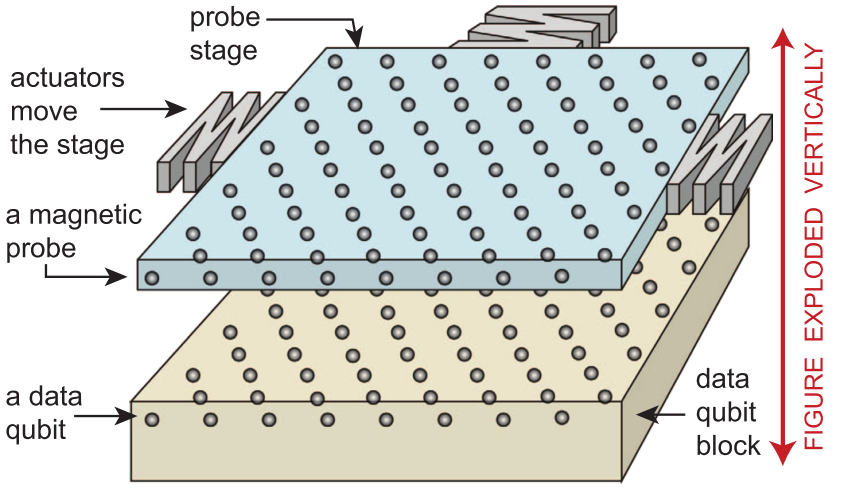
\includegraphics[width=0.8\linewidth]{../Figures/paper-mems} \label{FIG:paper-mems}}\\
	\subfloat[]{ 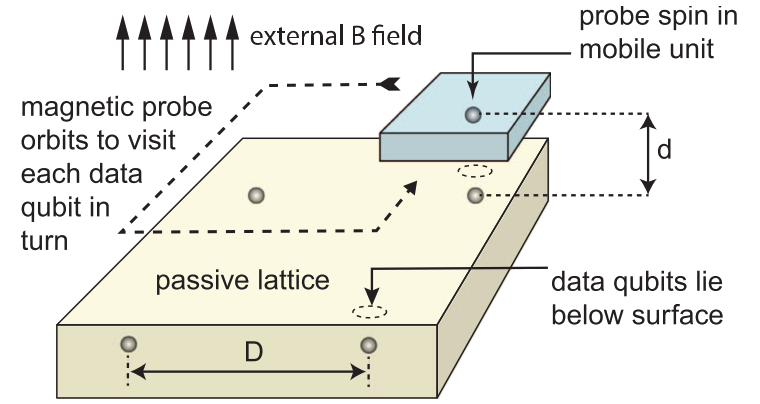
\includegraphics[width=0.8\linewidth]{../Figures/paper-parity} \label{FIG:paper-parity}}
	\caption[paper]{\textbf{(a)} Schematic of a scalable processor where data and ancillary/probe qubits are arranged in arrays in two different layers/stages which are moving relative to each other. \textbf{(b)} Magnified view of four data and one probe qubit. The movement results in the probe qubit orbiting above the data qubits allowing to implement a parity measurement. Direct copy from \cite{OGorman2016}.}
	\label{FIG:paper}
\end{figure}

This scheme requires a high precision in qubit placement. Therefore, \citet{OGorman2016} performed large-scale fault-tolerance simulation to obtain thresholds on the qubit placement precision. The orbit and movement can be performed in many different ways. They presented results for an abrupt orbit, where the probe qubit is moved rapidly from one data qubit to another, and a smooth, circular orbit.

Several thresholds were obtained with respect to the qubit placement precision where the data qubit displacement distribution takes either a `pillbox' (see fig.\@ \ref{fig:pillbox}) or an ellipsoid shape.
They found reasonable thresholds for each configuration compared to current qubit placement precisions offering good prospects for achieving logical qubit protection at the large scale. 

If we were to implement such a system in the lab, we would probably start with the smallest possible building block, which in this case is the system consisting of four data qubits and a single probe qubit to demonstrate a single parity measurement.



\subsection{Spin species}

Having demonstrated how the parity measurement is realised and how long each measurement could take we now look into different available spin systems. 

As shown in the previous sections we require $\Delta d^3/ J > 10^4$. This is achieved by choosing two different spin species for the data and probe qubits. Any sensible combination of species given in Table.\@ \ref*{TAB:qubits} fulfils this criterion.

For the data qubits we desire qubits with long coherence to maintain the quantum information throughout a large number of parity measurements. Furthermore, we only require global control for the data qubits during operation as logical operations on the encoded qubits can be performed using the stabilizer measurements.
In case of the probe qubits we require coherence times which are longer than the time it takes to perform a parity measurement. In addition to that readout is very important and individual control is required.


\begin{table}[H]
	\begin{tabular}{lrrrr}
		\hline
		spin qubit & $T_1$ & $T_2^{*}$ & $T_2$ & $T_{2,\textrm{decoupl}}$ \\ \hline \\
		P (nat. Si, mK, SET) \cite{Pla2012}& $0.7\, $s & $^{10}55\, $ns  & $^5206\, \si{\micro s}$ & $410\, \si{\micro s}$  \\
		P ($^{28}$Si, mK, SET) \cite{Muhonen2014}&  & $^7160\, \si{\micro s}$  & $^41\, $ms & $560\, $ms \\
		P$^{\text{nuc}}$ ($^{28}$Si, mK, SET) \cite{Muhonen2014}& & $500\, \si{\micro s}$ & $1.75\, $s & $35.6\, $s \\
		P ($^{28}$Si, $6.9\, $K, bulk) \cite{Morley2010}& &  & $14\, $ms &  \\
		P ($^{28}$Si, $1.8\, $K, bulk) \cite{Tyryshkin2011}& &  & $0.6\, $s &  \\
		Bi ($^{28}$Si, $4.3\, $K bulk CT) \cite{Wolfowicz2013} & $9\, $s &  & $^12.7\, $s &\\
		NV ($^{12}$C, RT) \cite{Balasubramanian2009,Bar-Gill2013} & & & $^21.8\, $ms & $3.3\, $ms \\
		NV ($^{12}$C, $77\, $K) \cite{Bar-Gill2013} & & &  & $0.6\, $s \\
		SiC ($20\, $K) \cite{Christle2014} & & $^81.1\, \si{\micro s}$ & $^31.2\, $ms &  \\
		SiC (RT) \cite{Koehl2011} & $185\, \si{\micro s}$ & $^9214\, $ns & $^640\, \si{\micro s}$ &   \\
		\hline
	\end{tabular} 
	\caption{Summary of coherence times of various spin qubit systems. The spin species as well as the measurement temperature is given. RT stands for room temperature while CT refers to clock transitions. For donors in Silicon we distinguish between near surface dopants read out using a single-electron-transistor (SET) and bulk dopants. The numbers in superscript refer to fig.\@ \ref{fig:phaseplot}.}
	\label{TAB:qubits}
\end{table}

This illustrates that coherence is an important parameter for choosing a spin system. Dephasing is a reversible loss of coherence due to inhomogeneous broadening which is characterised by the dephasing time $T_2^*$ which is usually much shorter than a millisecond (see Table.\@ \ref{TAB:qubits}). Luckily we should be able to combine the parity measurement with spin echo or even dynamical decoupling techniques enhancing coherence to the more generous time $T_2$ which represents irreversible loss of coherence.

Donors in silicon are excellent candidates for both data and probe qubits as they offer extremely long coherence times when implanted in purified $^{28}$Si (see Table.\@ \ref{TAB:qubits}). Moreover, electrical read out of high-fidelity using a single-eletron-transistor (SET) \cite{Pla2012,Pla2013,Muhonen2014} as well as optical \cite{Lo2015} read out has been demonstrated for $^{31}$P donors and is feasible for $^{209}$Bi. Control of individual spins can be achieved by tuning them in and out of resonance using the stark effect \cite{Pica2014}. The control electronics has a small footprint making a large scale implementation feasible. Being able to transfer the electron spin state to the nuclear spin offers even longer coherence times. Additionally, $^{209}$Bi has several clock transitions (CT) which are insensitive to magnetic fields leading to very long electron spin coherence times ($T_2=2.7\, $s). However, operation in this regime will make the $^{209}$Bi qubit also insensitive to the magnetic dipole-dipole interaction. Tuning in an out of the CT will be necessary to implement the parity measurement. Proof-of-concept implementations could benefit from that fact that donors in silicon even offer moderate coherence times at elevated temperatures. However, the coherence times demonstrated in bulk still remain to be reproduced for near-surface donors as required for this scheme.
Finally, MEMS devices with a sensitivity of \SI{25}{\hertz\per nm} and $0.3\, $nm accuracy \cite{Chu2003} as well as an accuracy of $5\, $nm with a bandwidth of $30\, $Hz have been demonstrated. This gives good prospects for realisation of highly accurate and fast MEMS devices as needed for this scheme in the near future. 

Besides donors in Si we imagine nitrogen vacancies (NV) to be a promising candidate for proof-of-concept demonstrations. NV centres are highly developed qubits \cite{Bar-Gill2013} which offer good coherence times even at room temperature (RT) \cite{Balasubramanian2009}. Individual addressing can be achieved using the stark effect. Optical read out and the possibility of integrating NV centres into an atomic force microscope (AFM) tip makes NV centres good candidates for a probe qubit \cite{Grinolds2013}. The optical read out of NV centres has one drawback as the readout frequency excites carriers in silicon. As a result of this read out has to be performed carefully in safe distance to the data qubits. Additionally diamond MEMS devices still need to be demonstrated.

Recently, defects in SiC have attracted lots of attention \cite{Morello2015} as coherent manipulation of individual spins with predicted room temeprature coherence times on the order of milliseconds has been demonstrated \cite{Widmann2014}. At cryogenic temperatures ($20\, $K) this has already been achieved \cite{Christle2014}. Current experiments still suffered from a low collection efficiency. Having near infra-red transitions, SiC shows excellent prospects for integration with optical fibres. Moreover, AFM tip integration is feasible. However, SiC is still at a very early research stage.  




\section{The Simulation}
In contrast to the large scale threshold analysis done by \citet{OGorman2016} this work focusses on the physical simulation of the building block of the surface code error detection - the stabilizer measurements which is done by measuring the parity of a group of qubits. On the smallest scale this is given by a group of four data qubits and one probe/ancillary qubit as shown in fig.\@ \ref{FIG:paper-parity}. 

\subsection{The dipole-dipole interaction}\label{sec:dipole-dipole}

The interaction of the orbiting ancillary qubit with each data qubit is governed by the following Hamiltonian:

\begin{equation*}
H = \mu_B B( g_1 \sigma_1^Z + g_2 \sigma_2^Z) + \frac{J}{r^3} ( \mathbf{\sigma_1} \cdot \mathbf{\sigma_2} - 3 ( \hat{\mathbf{r}} \cdot \mathbf{\sigma_1}) ( \hat{\mathbf{r}}\cdot \mathbf{\sigma_2}))
\end{equation*}

First of all, there is the Zeeman part which accounts for the energy of each spin (data and probe) in an external magnetic field. The interaction is of magnetic dipole-dipole type with the interactions strength $J=\frac{\mu_0 g_e^2 \mu_B^2}{4\pi}$ and $\hat{\mathbf{r}}$ is the unit vector between the two spins. The magnetic dipole-dipole interaction is of long range compared to proposals based on the exchange interaction \cite{Kane1998a} which makes this approach very attractive as it lowers the enormous requirements on the qubit placement precision as shown by \citet{OGorman2016}. Nevertheless, the interaction scales with $1/r^3$ which makes a data to probe qubit distance on the order of several tenths of nanometres necessary to achieve a strong interaction. In order to avoid crosstalk between the data qubits in the plane the lattice spacing $D$ of the data qubits should be at least one order of magnitude larger than the data and probe spacing $d$. 

Our goal is to achieve a parity measurement using this interaction. The dipole-dipole term allows us to do a controlled phase gate between the data and probe qubit which is shown in \cite{OGorman2016} and can be seen from the dependence on both spin matrices $\mathbf{\sigma_1}$ and $\mathbf{\sigma_2}$. This means that depending on the data qubit state the probe qubit evolves in a different direction on the bloch sphere (acquires a different phase). 

In order to simulate the time evolution of both qubits under the effect of this Hamiltonian by solving the Schr\"odinger or master equation we need to transform into the interaction picture and apply the rotating wave approximation. This allows us to get rid of the fast dynamics given by the Zeeman term while maintaining the physical interaction which we are interested in. In our work simulations have been done using the master equation solver provided by the QuTiP library in Python \cite{Johansson2012,Johansson2013}.

In this approximation the interaction Hamiltonian is given by:

\begin{align*}
	H_{int}&= \frac{J}{r^3} (1-3 \cdot \hat{r}_z^2) \cdot
	\begin{pmatrix}
	1 & 0 & 0 & 0 \\
	0 & -1 & 0 & 0 \\
	0 & 0 & -1 & 0 \\
	0 & 0 & 0 & 1 
	\end{pmatrix} \\
	&+ \frac{J}{r^3} (2-3 \cdot \hat{r}_x^2 -3 \cdot \hat{r}_y^2) \cdot
	\begin{pmatrix}
	0 & 0 & 0 & 0 \\
	0 & 0 & e^{-4 \Delta i} & 0 \\
	0 & e^{4 \Delta i} & 0 & 0 \\
	0 & 0 & 0 & 0 
	\end{pmatrix}
\end{align*}

Here $\Delta=\mu_B B (g_1-g_2)$. Depending on the relation between $\Delta$ and $J/r^3$ the interaction will have a different character. 
To achieve a controlled phase gate on the probe qubit while keeping the data qubit unchanged we want to be in the regime where $\Delta \gg J/r^3$.
In order to estimate what orders of magnitude we require to achieve this we performed simulations for various magnitudes of $\Delta d^3/ J$ where $d$ is the minimal interaction distance as shown in fig.\@ \ref{FIG:paper-parity}.

\begin{figure}[H]
	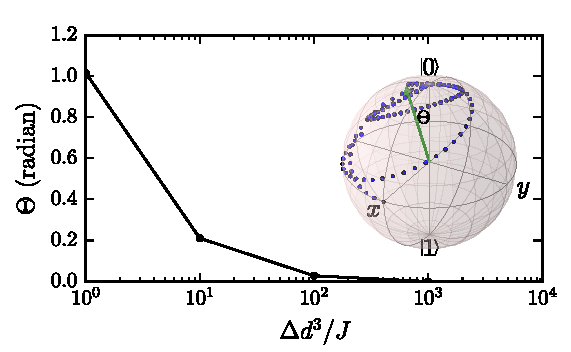
\includegraphics[width=\linewidth]{../Figures/flip-flop}
	\caption{Quantifying the flip-flopping character of the dipole-dipole interaction. For small $\Delta d^3/ J$ (see inset) we observe strong flip-flopping of the data and probe qubit which we show by plotting the maximum angle $\Theta$ which the data qubit (initialised in $\ket{0}$) takes throughout the evolution. We require $\Delta d^3/ J > 10^4$ to preserve the data qubit state.}
	\label{FIG:flip-flop}
\end{figure}

When $\Delta = J/d^3$ we observe a strong flip-flopping behaviour between the data (initialised in $\ket{0}$) and probe qubit (initialised in $\ket{+}$) as shown in the inset of fig.\@ \ref{FIG:flip-flop}. We want to avoid any change of the data qubit state. To quantify the flip-flopping we plot the angle theta the data qubit evolves for a given time for different magnitudes of $\Delta d^3/ J$ (see fig.\@ \ref{FIG:flip-flop}). Flip-flopping vanishes for $\Delta d^3/ J > 10^4$ preserving the data qubit state. This is achieved by using different species of qubits for the data and probe lattice (see Table. \ref{TAB:qubits}).

\subsection{The parity measurement}
Having identified the regime where the dipole-dipole interaction is able to perform a controlled-phase gate, we move on to the demonstration of a parity measurement.

The parity measurement should report 'even' when the number of data qubits pointing up and pointing down is even. And it should report 'odd' when the number of data qubits pointing up and pointing down is odd.

Realising a parity measurement using the controlled-phase gate is done by initialising the probe qubit in the $\ket{+}$ state and timing the interacting of the probe qubit with every data qubit such that the probe qubit acquires a controlled phase of $\pi/2$ for every data qubit. In case of even parity the probe qubit will then always evolve into the $\ket{+}$ state (see fig.\@ \ref{FIG:even} for the case of all four qubits being initialised in $\ket{0}$) while odd parity brings the probe qubit to the $\ket{-}$ state (see fig.\@ \ref{FIG:even} where one of the four qubits has been initialised in $\ket{1}$). The parity is therefore obtained by measuring the probe qubit in the $x$-basis.    


\begin{figure}[H]
	\subfloat[]{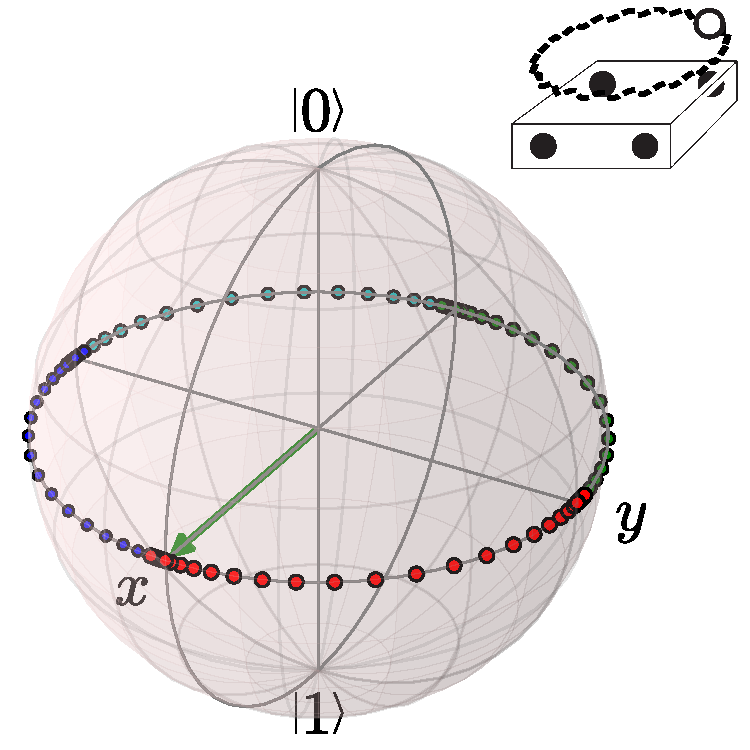
\includegraphics[width=0.49\linewidth]{../Figures/perfect_evolution_even_edit} \label{FIG:even}}
	\subfloat[]{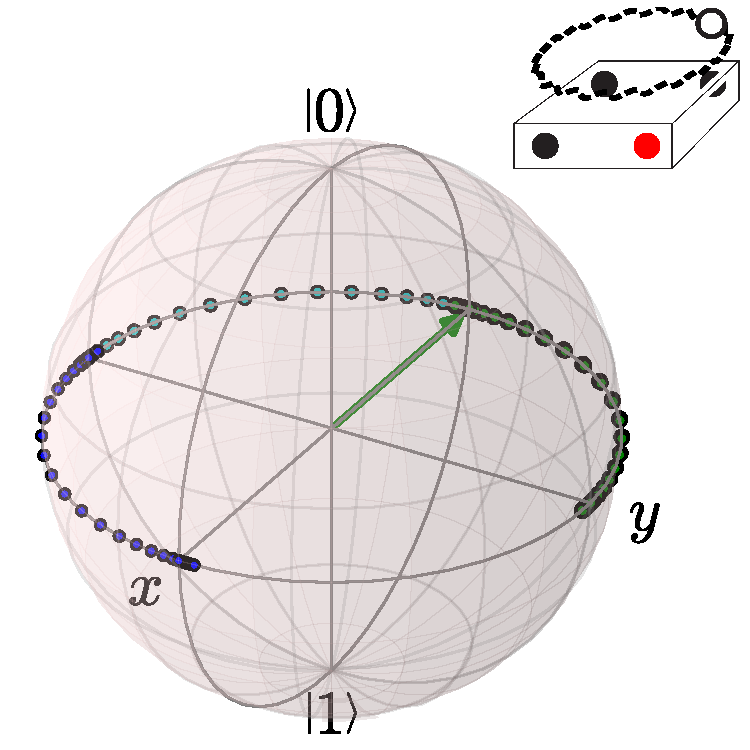
\includegraphics[width=0.49\linewidth]{../Figures/perfect_evolution_odd_edit} \label{FIG:odd}}
	\caption[oddeven]{Demonstration of the parity measurement using the controlled  $\pi/2$ phase gate and initialisation of the probe qubit in the $\ket{+}$ state. (a) All data qubits are initialised in the $\ket{0}$ state (black) representing an even parity configuration. The probe qubit undergoes a $2\pi$ evolution back to  the $\ket{+}$ state. (b) Now the last qubit is initialised in the $\ket{1}$ state (red). As a result of this the probe qubit evolves into the $\ket{-}$ state. Any other odd or even configuration will result in the same final state. The parity is extracted by measuring the probe qubit in the $x$-basis. The four different colours indicate the interaction with the four data qubits.}
	\label{FIG:evolution}
\end{figure}


The orbit which the probe qubits take to perform the parity measurement can take any possible form. Our simulations include an abrupt movement where the probe qubit jumps directly from one data qubit to the next and so on (see fig.\@ \ref{FIG:paper-abrupt}). This is very unphysical but describes the optimal orbit as it reduces the parity measurement time to a minimum. In addition to that we simulate a circular orbit with a constant speed (see fig.\@ \ref{FIG:paper-circ}). An intermediate orbit between these two extreme cases will most likely be implemented in an experiment. 

The time each data qubit should interact with the probe qubit to realise a controlled $\pi/2$ rotation in the bloch sphere is obtained by varying the interaction time while monitoring the phase acquired by the probe qubit. This is done for every chosen orbit and an exemplary simulation is shown in fig.\@ \ref{FIG:get_tau} for the abrupt orbit. A rotation of $\pi/2$ is achieved for $\tau\approx 77\, \mu$s.

\begin{figure}[H]
	\begin{minipage}[t]{0.15\linewidth} 
	\subfloat[]{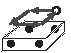
\includegraphics[width=\linewidth]{../Figures/abrupt} \label{FIG:paper-abrupt}}\\
	\subfloat[]{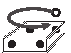
\includegraphics[width=\linewidth]{../Figures/circ} \label{FIG:paper-circ}}
	\end{minipage}
	\subfloat[]{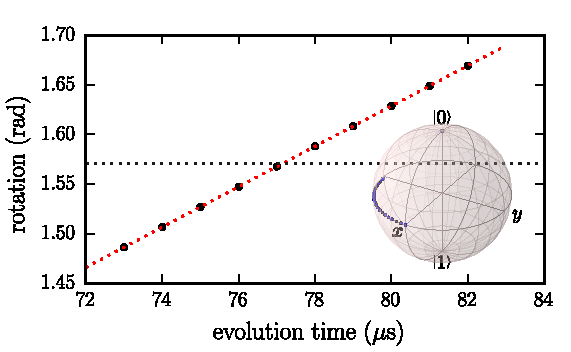
\includegraphics[width=0.85\linewidth]{../Figures/abrupt_find_tau_full.pdf} \label{FIG:get_tau}}
	\caption{(a) Schematic of the abrupt orbit. Direct copy from \cite{OGorman2016}. (b) Schematic of the circular orbit. Direct copy from \cite{OGorman2016}. (c) We obtain the optimal interaction duration to implement a $\pi/2$ rotation by varying the evolution time while monitoring the phase acquired by a probe qubit initialised in the $\ket{+}$ state. Here we show the example of the abrupt orbit with $d=40\, $nm and we find $\tau\approx 77\, \mu$s.}
	\label{FIG:abrupt_tau}
\end{figure}

In order to estimate the time a parity measurement would take in an experiment, we determine the parity measurement time for the abrupt and circular orbit for several data and probe qubit separations $d$ and data qubit lattice spacings $D$.

\begin{figure}[H]
	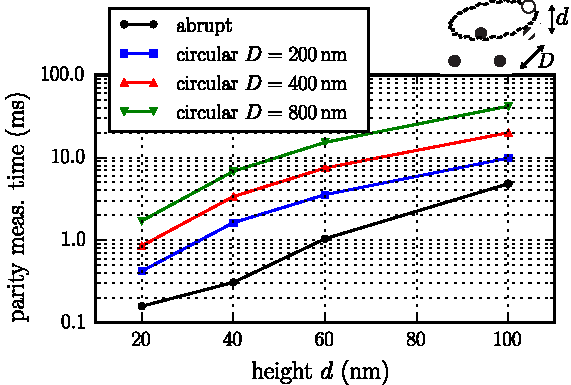
\includegraphics[width=\linewidth]{../Figures/tau_d_D}
	\caption{Simulation of the overall parity measurement time for the abrupt and circular orbit with various qubit lattice constants $D$ and probe and data qubit layer separation $d$.}
	\label{FIG:tau}
\end{figure}

The shortest parity measurement time $\tau=158\, \mu$s is achieved with the abrupt motion ($d=20\, $nm).
The parameter $d$ has the strongest influence on the parity measurement time due to the $1/r^3$ dependence of the interaction.
For a reasonable experimental implementation, we expect the parity measurement to be of the order of several milliseconds.


\subsection{Spin species}

Having demonstrated how the parity measurement is realised and how long each measurement could take we now look into different available spin systems. 

As shown in the previous sections we require $\Delta d^3/ J > 10^4$. This is achieved by choosing two different spin species for the data and probe qubits. Any sensible combination of species given in Table.\@ \ref*{TAB:qubits} fulfils this criterion.

For the data qubits we desire qubits with long coherence to maintain the quantum information throughout a large number of parity measurements. Furthermore, we only require global control for the data qubits during operation as logical operations on the encoded qubits can be performed using the stabilizer measurements.
In case of the probe qubits we require coherence times which are longer than the time it takes to perform a parity measurement. In addition to that readout is very important and individual control is required.


\begin{table}[H]
	\begin{tabular}{lrrrr}
		\hline
		spin qubit & $T_1$ & $T_2^{*}$ & $T_2$ & $T_{2,\textrm{decoupl}}$ \\ \hline \\
		P (nat. Si, mK, SET) \cite{Pla2012}& $0.7\, $s & $^{10}55\, $ns  & $^5206\, \si{\micro s}$ & $410\, \si{\micro s}$  \\
		P ($^{28}$Si, mK, SET) \cite{Muhonen2014}&  & $^7160\, \si{\micro s}$  & $^41\, $ms & $560\, $ms \\
		P$^{\text{nuc}}$ ($^{28}$Si, mK, SET) \cite{Muhonen2014}& & $500\, \si{\micro s}$ & $1.75\, $s & $35.6\, $s \\
		P ($^{28}$Si, $6.9\, $K, bulk) \cite{Morley2010}& &  & $14\, $ms &  \\
		P ($^{28}$Si, $1.8\, $K, bulk) \cite{Tyryshkin2011}& &  & $0.6\, $s &  \\
		Bi ($^{28}$Si, $4.3\, $K bulk CT) \cite{Wolfowicz2013} & $9\, $s &  & $^12.7\, $s &\\
		NV ($^{12}$C, RT) \cite{Balasubramanian2009,Bar-Gill2013} & & & $^21.8\, $ms & $3.3\, $ms \\
		NV ($^{12}$C, $77\, $K) \cite{Bar-Gill2013} & & &  & $0.6\, $s \\
		SiC ($20\, $K) \cite{Christle2014} & & $^81.1\, \si{\micro s}$ & $^31.2\, $ms &  \\
		SiC (RT) \cite{Koehl2011} & $185\, \si{\micro s}$ & $^9214\, $ns & $^640\, \si{\micro s}$ &   \\
		\hline
	\end{tabular} 
	\caption{Summary of coherence times of various spin qubit systems. The spin species as well as the measurement temperature is given. RT stands for room temperature while CT refers to clock transitions. For donors in Silicon we distinguish between near surface dopants read out using a single-electron-transistor (SET) and bulk dopants. The numbers in superscript refer to fig.\@ \ref{fig:phaseplot}.}
	\label{TAB:qubits}
\end{table}

This illustrates that coherence is an important parameter for choosing a spin system. Dephasing is a reversible loss of coherence due to inhomogeneous broadening which is characterised by the dephasing time $T_2^*$ which is usually much shorter than a millisecond (see Table.\@ \ref{TAB:qubits}). Luckily we should be able to combine the parity measurement with spin echo or even dynamical decoupling techniques enhancing coherence to the more generous time $T_2$ which represents irreversible loss of coherence.

Donors in silicon are excellent candidates for both data and probe qubits as they offer extremely long coherence times when implanted in purified $^{28}$Si (see Table.\@ \ref{TAB:qubits}). Moreover, electrical read out of high-fidelity using a single-eletron-transistor (SET) \cite{Pla2012,Pla2013,Muhonen2014} as well as optical \cite{Lo2015} read out has been demonstrated for $^{31}$P donors and is feasible for $^{209}$Bi. Control of individual spins can be achieved by tuning them in and out of resonance using the stark effect \cite{Pica2014}. The control electronics has a small footprint making a large scale implementation feasible. Being able to transfer the electron spin state to the nuclear spin offers even longer coherence times. Additionally, $^{209}$Bi has several clock transitions (CT) which are insensitive to magnetic fields leading to very long electron spin coherence times ($T_2=2.7\, $s). However, operation in this regime will make the $^{209}$Bi qubit also insensitive to the magnetic dipole-dipole interaction. Tuning in an out of the CT will be necessary to implement the parity measurement. Proof-of-concept implementations could benefit from that fact that donors in silicon even offer moderate coherence times at elevated temperatures. However, the coherence times demonstrated in bulk still remain to be reproduced for near-surface donors as required for this scheme.
Finally, MEMS devices with a sensitivity of \SI{25}{\hertz\per nm} and $0.3\, $nm accuracy \cite{Chu2003} as well as an accuracy of $5\, $nm with a bandwidth of $30\, $Hz have been demonstrated. This gives good prospects for realisation of highly accurate and fast MEMS devices as needed for this scheme in the near future. 

Besides donors in Si we imagine nitrogen vacancies (NV) to be a promising candidate for proof-of-concept demonstrations. NV centres are highly developed qubits \cite{Bar-Gill2013} which offer good coherence times even at room temperature (RT) \cite{Balasubramanian2009}. Individual addressing can be achieved using the stark effect. Optical read out and the possibility of integrating NV centres into an atomic force microscope (AFM) tip makes NV centres good candidates for a probe qubit \cite{Grinolds2013}. The optical read out of NV centres has one drawback as the readout frequency excites carriers in silicon. As a result of this read out has to be performed carefully in safe distance to the data qubits. Additionally diamond MEMS devices still need to be demonstrated.

Recently, defects in SiC have attracted lots of attention \cite{Morello2015} as coherent manipulation of individual spins with predicted room temeprature coherence times on the order of milliseconds has been demonstrated \cite{Widmann2014}. At cryogenic temperatures ($20\, $K) this has already been achieved \cite{Christle2014}. Current experiments still suffered from a low collection efficiency. Having near infra-red transitions, SiC shows excellent prospects for integration with optical fibres. Moreover, AFM tip integration is feasible. However, SiC is still at a very early research stage.  


 


\section{Errors} \label{sec:errors}
In this section, we will present three types of errors that we implement in the simulation: path jitter, dephasing and data qubit displacement. Path jitter influences the probe qubit orbit ($r$ in the Hamiltonian), whereas dephasing is introduced into the master equation through a Lindblad operator. Finally, we simulated data qubit displacement by adding a random offset for each of the four data qubits of one orbit. In connection to qubit displacement, we will also review a technique called \emph{twirling} which averages out the effect of displacement errors. Before we do so, however, we must first make explicit which errors we are concerned with and how we can quantify the performance of the system. 


\subsection{Benchmarking}
In our simulation, there are two significant ways to quantify errors, and we shall quickly review them as they will be used extensively in the following sections.

The first way to quantify an error is to look at the phase $\phi$ accumulated by the probe qubit through the interaction with the data qubits. \citet{OGorman2016} present a general phase jitter as a collective error for randomness in the interaction which is defined as $\phi + \delta$, where $\delta$ is a small deviation from $\frac{\pi}{2}$.  In the paper, it was found that a phase jitter of $4.4 \%$ did not have a substantial impact on the fault-tolerance threshold. We will therefore attempt to compare the phase error in our simulation with this value whenever possible. It should be noted, however, that the data we have access to usually concerns the entire run. We will therefore compare the phase error with $2\pi$ or $\pi$. We have made the assumption that the phase error for one quarter run stacks, such that after the full orbit the phase error of $\frac{\pi}{2}$ is the same percentage as the phase error of $2\pi$ that we observe. 

The second way to quantify errors is to look at the probability of correctly identifying the stabiliser state  $\ket{\psi}$ through measurement of the probe qubit. As already mentioned, the outcome of the stabiliser measurement depends on whether we find $\ket{\psi}$ to be either in the $\ket{+}$ state or the $\ket{-}$ state. The probability $p$ is given by $|\braket{+|\psi}|^2$ in the case of an even parity measurement and $|\braket{- |\psi}|^2$ in the case of an odd parity measurement. The need for this measure arises for example when we introduce a dephasing term in the Lindblad equation. A dephasing operator will not cause any phase error to appear since dephasing only decreases the magnitude of the Bloch vector and not its direction. Therefore, the probability $p_{\textrm{succ}}$ of successfully identifying the stabiliser state becomes a good indicator of performance. It ranges from $p_{\textrm{succ}} = 1$ when the probe qubit state is completely pure and without phase error to $p_{\textrm{succ}} = 0.5$ when the state has completely decohered and the stabiliser measurement becomes inherently random. 

With these two measures in mind, let us look at the errors we introduced into the simulation and their effect on the performance of the system. 




%\clearpage
\subsection{Path Jitter}\label{sec:jitter}
The first error that we shall introduce is a jitter present in the orbit performed by the probe qubit. The precision provided by modern MEMS control structures depends on the speed we want to operate them at \cite{Chu2003,Koo2012}. Improvements are needed to implement a $1\, $kHz operation (which corresponds to the expected parity measurement time) with near $1\, $nm precision but we expect developments in the near future. Nevertheless, adding some random path jitter into the simulation will give us a good picture of what kind of error we can expect. At first, we attempted to simulate random jumps in the trajectory, but the discontinuities led to large derivative terms which in turn caused the simulation to fail. Thus,  we instead superposed a sinusoidal motion onto the trajectory path. To ensure that we see some randomness in the motion, we varied the phase with which the sinusoidal motion starts. The amplitude of the motion represents the largest jitter errors on the scale of nanometres. The results can be found in Figure \ref{fig:pathjitter}, where we note that an uncertainty of about 2 nm is sufficient for staying below the phase error threshold of $4.4 \%$. Note that we are not comparing the phase jitter with the measurement probability since the probe qubit is not undergoing dephasing due to this interaction. Furthermore, it is sufficient to look at jitter in the $y$-direction instead of both the $x$ and $y$ direction, since the phase error is symmetric between them. 
From the graph it also becomes clear that jitter in the $z$-direction has the greatest influence. This is due to the $\frac{1}{r^3}$  term in the Hamiltonian.



\begin{figure}[h]
  \centering
    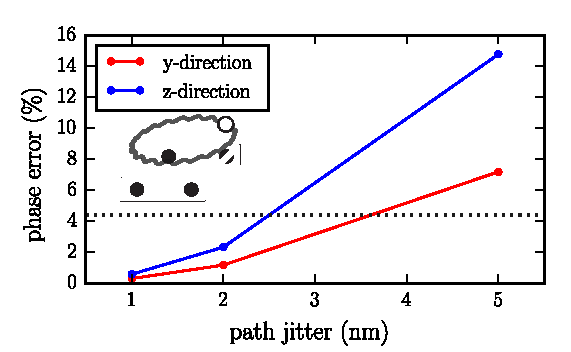
\includegraphics[width=0.5\textwidth]{../Figures/path_jit.pdf}
      \caption{Graph representing the percentage of phase error as a function of phase jitter in the $y$-direction (red) and in the $z$-direction (blue). There is a stronger dependence in the $z$-direction due to the $1/r^3$ term in the Hamiltonian.}
      \label{fig:pathjitter}
\end{figure}







\subsection{Dephasing}
Next, we investigated the influence of dephasing on the measurement probabilities. In order to simulate dephasing, which is the gradual reduction of the Bloch vector in the $x$--$y$ plane towards the origin of the Bloch sphere, we introduced a Lindblad operator into the master equation. The operator is given by 
\beq
L  = \sqrt{\Gamma} \sigma_z,
\eeq
where $\Gamma$ is the dephasing parameter, which can also be written as $1/T$ where $T$ is the dephasing time. In figure \ref{FIG:abr-deph}, we show the effects of a dephasing time of $1.2\, $ms given an abrupt orbit, and in figure \ref{FIG:circ-deph} we show the effects of the same dephasing time of $1.2\, $ms for a circular orbit. In the latter case, the probe first sits far away from the data qubit, where the interaction is weak and the only evolution to its state is the dephasing. Then, as it moves closer, the interaction gets stronger very rapidly, after which the probe qubit will again undergo an evolution with weak interaction experiencing dephasing. Due to the longer time required for the circular orbit, it is clear that dephasing has a much more severe impact on the probe state in the circular orbit than the abrupt orbit. 

\begin{figure}[H]
	\subfloat[]{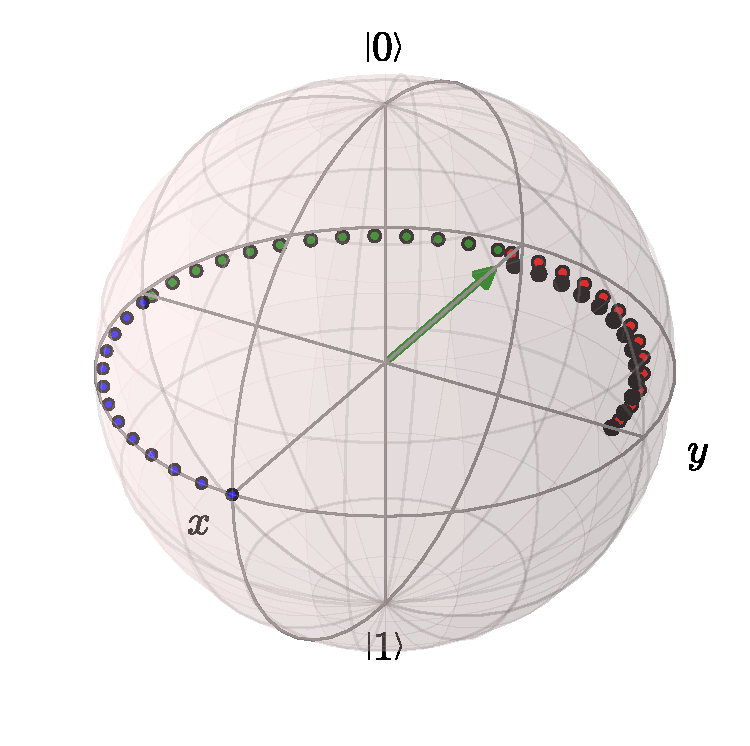
\includegraphics[width=0.49\linewidth]{../Figures/abrupt-deph} \label{FIG:abr-deph}} 
	\subfloat[]{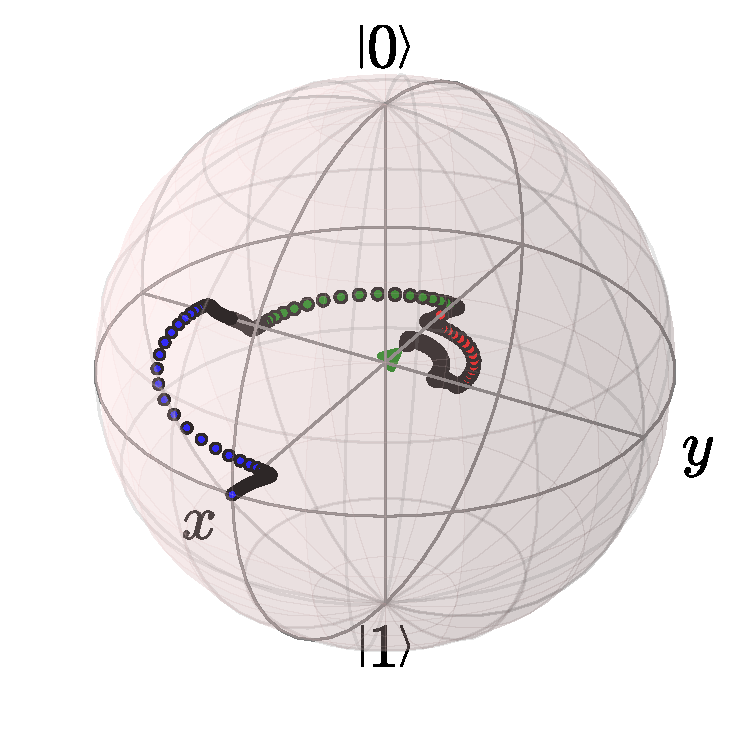
\includegraphics[width=0.49\linewidth]{../Figures/circ-deph} \label{FIG:circ-deph}}
	\caption[oddeven]{The evolution of the probe qubit state plotted in the Bloch sphere for a dephasing time $1.2\, $ms where one of the data qubits contains an error. The phase of the probe qubit is not affected since no relaxation or excitation is taking place. The effect can however be seen in the probability of measuring the probe qubit in the $\ket{+}$ or $\ket{-}$ state. \textbf{(a)} shows the dephasing for an abrupt orbit and \textbf{(b)} shows the dephasing for a circular orbit.}
	\label{FIG:deph}
\end{figure}


However, since dephasing does not affect the phase accumulated after the full run, we do not end up with a phase error. Therefore, the only accurate measure of errors due to dephasing is the probability of correctly identifying the probe qubit in either the $\ket{+}$ (even parity) or $\ket{-}$ (odd parity) states. We ran simulations for both the abrupt and circular orbit using the $T_2$ and $T_2^*$ values given in Table \ref{TAB:qubits} as input parameters for the dephasing time. The results can be seen in Figure \ref{fig:dephasingplot}, where each data point refers to an entry in the table. 

We can compare the probability of correctly measuring the stabiliser in the $\ket{-}$ state with the surface code fault-tolerance threshold of $1.1\%$, taking the failure to measure the stabiliser as the worst-case scenario probability (that is, assuming that all other errors occur with lower probability). Looking at the values displayed in Figure \ref{fig:dephasingplot}, we find that only the clock transition in bismuth leaves us within the fault-tolerance threshold. For the circular orbit, bismuth $(1)$ has a success probability of  99.9\% after one entire run.  The next best value is obtained for NV centres at room temperature $(2)$ which give us a success probability of 57.7\% in the case for the circular orbit, and 92.1\% for the abrupt orbit. Both of these probabilities are below the surface code threshold. 

We see that the clock transition in bismuth does exceptionally well, but that many spin species decohere long before the run is complete. This is especially clear in the case for the circular orbit, which takes approximately $10$ times longer than the abrupt orbit. It should be noted however that values of the  $T_2^*$ time in the graph were measured without the aid of Hahn echoes \cite{levitt1979nmr} or dynamical decoupling \cite{viola1998dynamical}. Therefore, these values should not be seen as representative, as these effects can be countered by implementing Hahn echoes or dynamic decoupling. Note that any echo technique would have to be applied on both the probe qubit and the data qubit as to preserve the direction of the evolution. 

As we discuss in more detail in Section \ref{sec:conclusions}, the impact of dephasing could be decreased by lowering the time needed for the probe qubit to complete one orbit around the data qubits. This would require lowering the distance $d$ between the probe qubits and the data qubits as to increase the interaction strength between them. 














\begin{figure}[h]
	\centering
	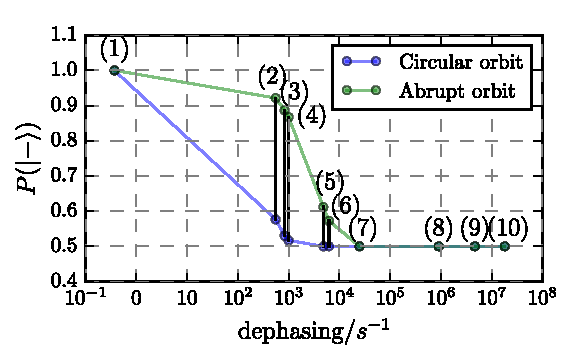
\includegraphics[width=1.05\linewidth]{../Figures/dephasing.pdf}
		\caption{A graph showing the relationship between the dephasing parameter $\Gamma$ and the probability $P(\ket{-})$ of measuring the probe qubit in the $\ket{-}$ state.  The blue data points represent an abrupt orbit and the green data points a circular orbit. Each number refers to a dephasing time found in Table \ref{TAB:qubits}. }
		\label{fig:dephasingplot}
\end{figure}








\subsection{Data qubit displacement}
The proposal \cite{OGorman2016} as described in section \ref{sec:PhysicalImplementation} utilises two distinct qubit arrays each of lattice constant $D$, separated by a distance $d$ perpendicular to the planes. To achieve reasonable interaction times compared to qubit decoherence times, distances $D = \SI{400}{\nano\metre}$ and $d = \SI{40}{\nano\metre}$ have been chosen for simulation.

It is may prove unrealistic, however, to expect to be able to deterministically place qubits with \si{\nano\metre} precision in a scalable manner. Resolutions of \SI{10}{\nano\metre} can be achieved using e-beam lithography \cite{Vieu2000a} or nanostencil masks \cite{Weis2008}, combined with single-ion implantation techniques \cite{Jamieson2005}. STM patterning techniques offer atomic precision of dopants in Si \cite{Schofield2003} but a method of maintaining this precision over an array several \si{\micro\metre} across remains elusive. 

To consider in detail the effect of these displacements, we generated uniformly random offsets to the position of each data qubit within a pillbox of heigh and radius $R$, as illustrated in fig.\@ \ref{fig:pillbox}. This form of displacement is the same as used in the proposal \cite{OGorman2016} and was chosen as the displacement in the $x$--$y$ plane would be expected to be uniformly radial, and the implantation depth in the $z$-axis would be independent from this.

To illustrate the errors qubit displacement creates, consider a set of typical qubit displacements as illustrated in fig.\@ \ref{fig:qubitdisplacements}. These displacements give each data qubit a different distance $r$ at which it is closest to the probe qubit as it passes overhead, resulting in a different interaction strength. Hence the phase accumulated for each data qubit varies from the ideal $\tfrac{\pi}{2}$ by an independent amount. These errors are systematic in that the same phases are picked up for each parity measurement, unlike the probe jitter considered in section \ref{sec:jitter}.

We find that for these displacements, the case of even parity (no bit-flips) yields close to a $2\pi$ evolution with $99.968\%$ probability of successfully measuring $\ket{+}$, from the evolution shown in fig.\@ \ref{fig:displacementnoerrors}. However, on introducing bit-flip errors to each of the four data qubits, different phase accumulations are observed as in fig.\@ \ref{fig:displacementerrors}.


\begin{figure}
	%\centering
	\begin{minipage}[t]{0.515\linewidth}
		\begin{flushleft}
		\subfloat[]{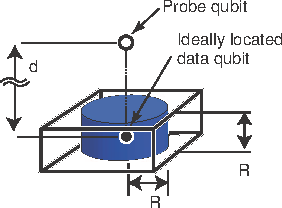
\includegraphics[width=0.6\linewidth]{../Figures/pillbox.pdf} \label{fig:pillbox}}\\
		\subfloat[]{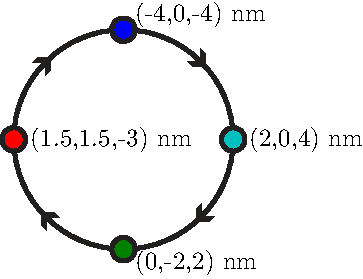
\includegraphics[width=0.7\linewidth]{../Figures/qubit_displacement_colours.pdf} \label{fig:qubitdisplacements}}
		\end{flushleft}
	\end{minipage}%
	\begin{minipage}[t]{0.485\linewidth}
	\subfloat[]{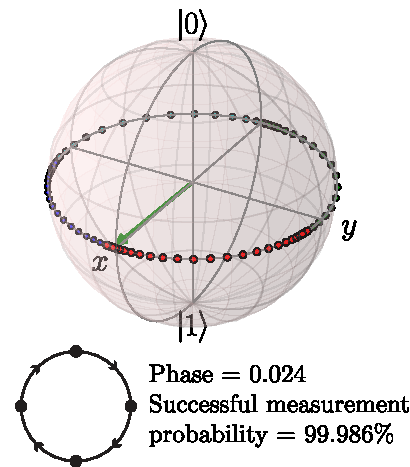
\includegraphics[width=\columnwidth]{../Figures/notwirl_noerror.pdf} \label{fig:displacementnoerrors}}
	\end{minipage}%
	
	\subfloat[]{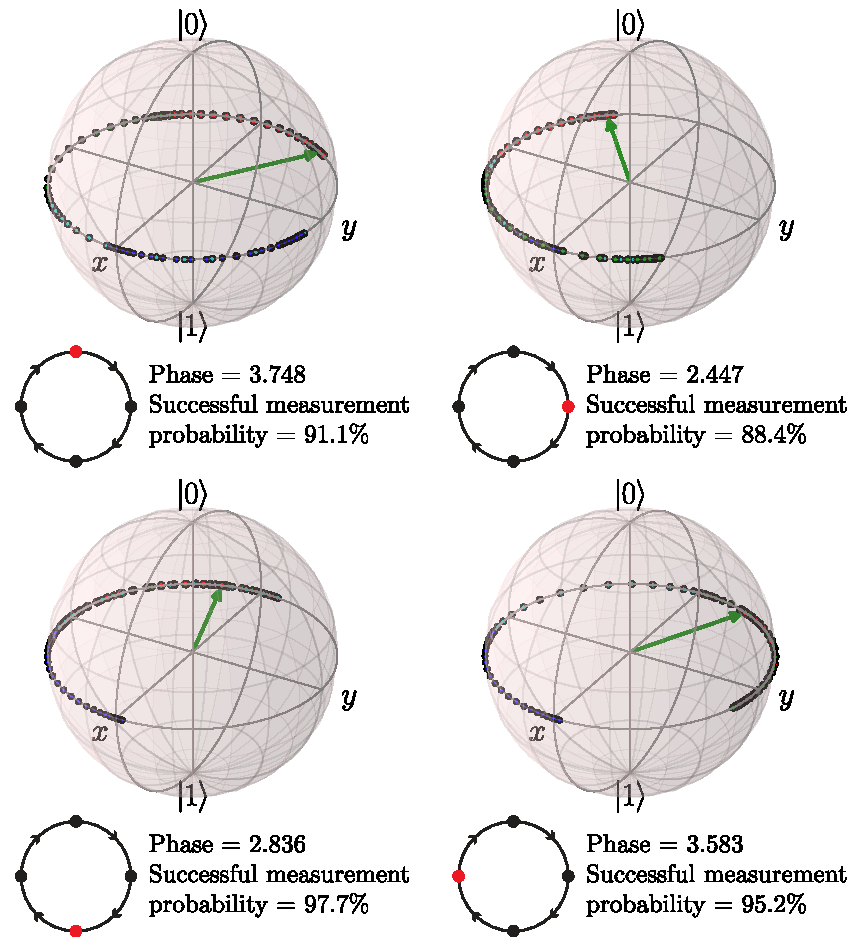
\includegraphics[width=1\columnwidth]{../Figures/notwirl_allerrors_portrait.pdf} \label{fig:displacementerrors}}
	
	\caption{Qubits displaced from the ideal lattice position give a phase contribution different to the ideal $\tfrac{\pi}{2}$ per qubit. (a) The pillbox region within which qubit displacements are randomly generated. Subfigure adapted from \cite{OGorman2016}. (b) The set of qubit displacements used to investigate the effects of displacement and twirling operations. (c) The phase accumulated and success probability for the displacements of (b) for even parity (no bit-flips). (c) The phase accumulated and success probability for each bit-flip error. Note the measurement success probability depends on which qubit is flipped, making the code susceptible to logical errors over repeated parity measurements. NOTE: change last subfigure to .pdf}
\end{figure}

%\begin{figure*}
%	\centering
%%	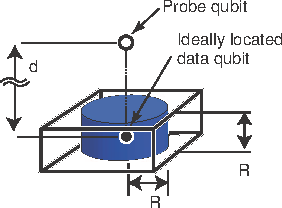
\includegraphics[width=\columnwidth]{../Figures/pillbox.pdf}
%	\subfloat[]{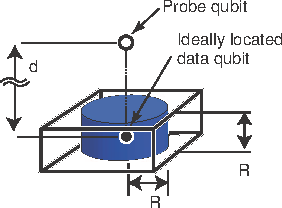
\includegraphics[width=0.7\columnwidth]{../Figures/pillbox.pdf} \label{fig:pillbox}}
%	\subfloat[]{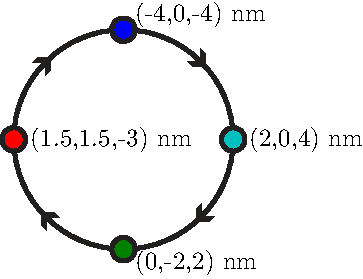
\includegraphics[width=0.7\columnwidth]{../Figures/qubit_displacement_colours.pdf} \label{fig:qubitdisplacements}}
%	\subfloat[]{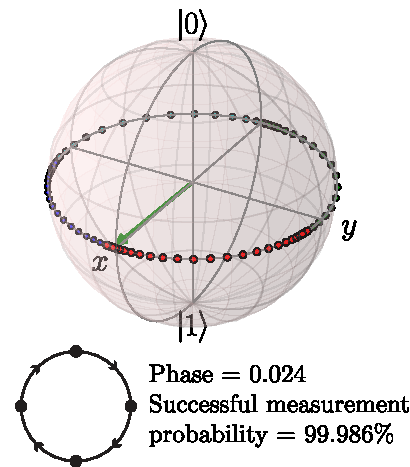
\includegraphics[width=0.5\columnwidth]{../Figures/notwirl_noerror.pdf} \label{fig:displacementnoerrors}}
%	
%	\subfloat[]{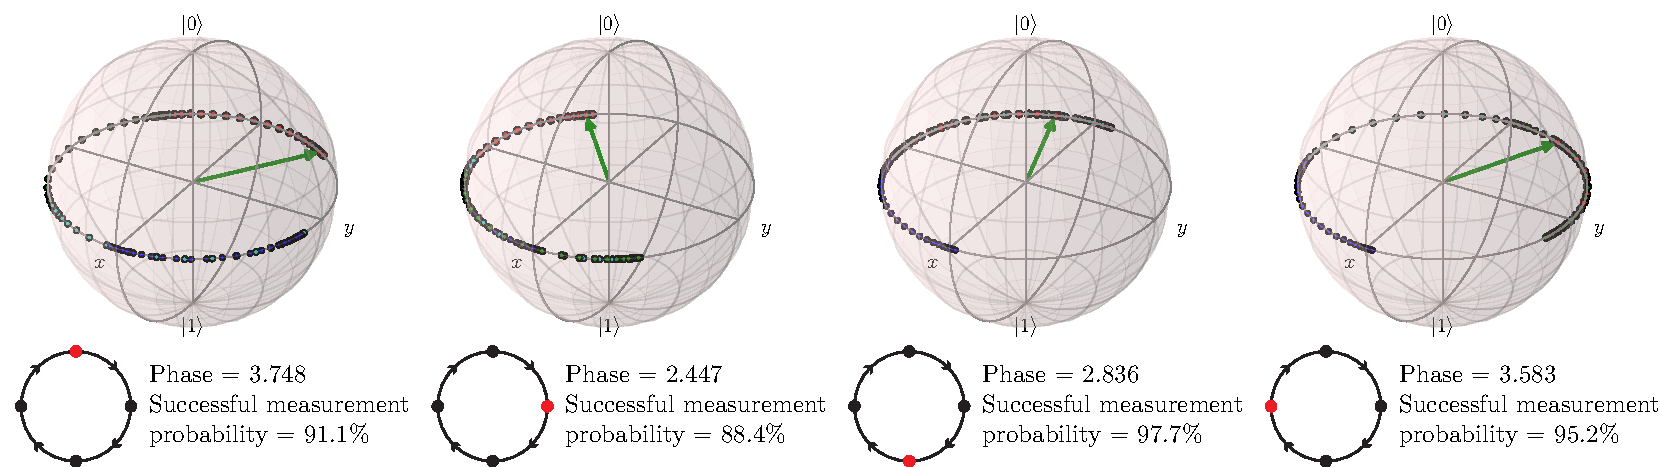
\includegraphics[width=2\columnwidth]{../Figures/notwirl_allerrors_landscape.pdf} \label{fig:displacementerrors}}
%	
%	\caption{Qubits displaced from the ideal lattice position give a phase contribution different to the ideal $\tfrac{\pi}{2}$ per qubit. (a) The pillbox region within which qubit displacements are randomly generated. Subfigure adapted from \cite{OGorman2016}. (b) The set of qubit displacements used to investigate the effects of displacement and twirling operations. (c) The phase accumulated and success probability for the displacements of (b) for even parity (no bit-flips). (c) The phase accumulated and success probability for each bit-flip error. Note the measurement success probability depends on which qubit is flipped, making the code susceptible to logical errors over repeated parity measurements. NOTE: change last subfigure to .pdf}
%\end{figure*}








\subsubsection{Twirling}

It is not the fact that the success probabilities are lower for odd parities than for even parity that is especially concerning; this is what fault-tolerant codes are designed to cope with. Instead it is the fact that bit-flips on each qubit give a \emph{different} probability of successful detection. This means one qubit will be more prone to undetected errors than others. The fault tolerance required by the proposal assumes a symmetry between the data qubits that this breaks, making the code susceptible to logical errors.

A method proposed to account for this is suggested in the proposal \cite{OGorman2016}. Their \emph{`twirling'} technique smooths out this asymmetry between data qubits by effectively switching the location of bit-flips randomly so that the phase accumulated due to any one bit-flip is on average the same as for any other bit-flip. This is done by randomly applying one of four unitary operations $\mathrm{U_1 = \op{I}\op{I}\op{I}\op{I}}$, $\mathrm{U_2 = \op{I}\op{I}\op{X}\op{X}}$, $\mathrm{U_3 = \op{I}\op{X}\op{I}\op{X}}$, $\mathrm{U_4 = \op{I}\op{X}\op{X}\op{I}}$, as illustrated in fig. \ref{fig:twirls}, both before and after the parity measurement.

This has the effect of making the average projection onto the $x$-axis the same for all odd parity cases as desired, at the expense of reduced success probability for even parity. This risks introducing Pauli errors \cite{OGorman2016} but provided the success probability is sufficiently high this is correctable by the code.


\begin{figure}
	\centering
	\subfloat[]{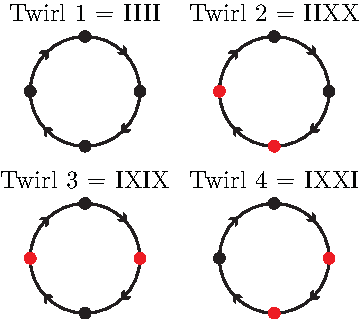
\includegraphics[width=0.4\columnwidth]{../Figures/twirls.pdf} \label{fig:twirls}}\hspace{0.05\columnwidth}
	\subfloat[]{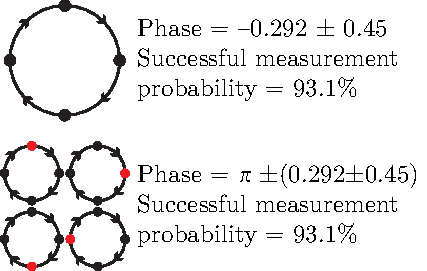
\includegraphics[width=0.5\columnwidth]{../Figures/twirl_effect.pdf} \label{fig:twirleffect}}
	\caption{`Twirling' operations. (a) Each of the four twirling operations which, when applied with equal probability, randomly change which qubit effectively contributes to odd parity, smoothing out asymmetries in success probabilities due to qubit displacements. (b) Effect on success probabilities for the displacements shown in fig.\@ \ref{fig:qubitdisplacements}. Even parity shows a reduction in success probability, while the success of odd parity measurements becomes constant on average.}
\end{figure}


\section{Conclusions and outlook } \label{sec:conclusions}
In this report, we we have presented results obtained from simulating a system of one probe qubit and four data qubits based on the setup proposed in \cite{OGorman2016}. We investigated how physically motivated errors affected the performance of the system and were able to determine the desired values for certain experimental parameters. 

We found that the ratio between the coupling constant $J$ and the detuning $\Delta$ should be of the order $\Delta r^3/J \ge 10^4$ to avoid flip-flopping of the data qubits. Furthermore, we characterised the impact of changing physical parameters, such as the separation between the probe and data qubits $d$ and the in-plane qubit lattice constant $D$ on the parity measurement time.  
Looking at the introduction of errors, our results show that path jitter has little effect on the overall performance, meaning that the resulting path jitter stays within the $4.4\%$ threshold set out in \cite{OGorman2016}. On the other hand, we find that dephasing has a strong influence on the success probability $p_{succ}$ of measuring the probe qubit in the correct state. Assuming that $p_{succ}$ is the largest of all probabilities for failure, out of all spin species we investigated, only bismuth was found to have dephasing times short enough to push $p_{succ}$ above the surface code threshold. Furthermore, introducing a random displacement in the position of the data qubits yielded $p_{succ} = 98.? \%$, which  again is above the surface code threshold. These results are obtained even when using values for the displacement error that are below the thresholds, as shown in \cite{OGorman2016}. One is however right to question whether the comparison between our results and those obtained by O'Gorman \textit{et al}. hold. Whereas they are looking at the fault-tolerance of an entire system, we are investigating the stabiliser measurement in isolation. One could simply compensate for the failing stabiliser by performing the measurement twice or trice, although this would severely increase the time required for each error-correcting step. More investigation is needed to see whether the effect of the data qubit displacement is as severe as shown here. 






As to how the project can be continued, there are many avenues that are worthy of investigation. We wrote the code for simulating qubit initialisation errors, but were unable to investigate the resulting effect due to constraints on computational time. Another rather natural extension is to combine the errors presented above and see how they affect the total performance. Even so, the dephasing time is likely to be the single most important factor that influences the probability of successfully distinguishing the probe qubit state. Therefore, it is imperative that we explore ways to decrease the impact of dephasing. We can identify many ways to do so, some already mentioned in Section \ref{sec:dephasing}. The first would be to investigate whether the full orbit measurement can be performed in a shorter time, especially in the case of the circular orbit. This can be done by decreasing the separation $d$ between the probe and data qubits or by decreasing the lattice parameter $D$ of the data and probe qubits. A shorter parity measurement time could also be achieved by speeding the probe qubit orbit up when being far away from the data qubits. 
There are however two limit factors in these approaches. The first is that the speed and precision achievable by the MEMS will be limited. Current MEMS will not be able to achieve near $1\, $nm precision at a speed of $1\, $kHz \cite{Koo2012,Chu2003} but we are optimistic about improvements in the near future. The second is whether the increased proximity to other data qubits induces interference and cross-talk between the probe qubit and other, neighbouring data qubits. 
An alternative to decreasing the time for one cycle is to tune the probe qubits in and out of a protected states such as clock transitions for bismuth or nuclear spin states (see Table.\@ \ref{TAB:qubits}). In Figure \ref{fig:dephasing} we saw that the clock transition in bismuth has a long dephasing time as it is protected from magnetic field noise. However, this makes the transition insensitive to any qubit interaction making it necessary to tune the probe qubit in and out of the clock transition to perform the parity measurement. The feasibility of this tuning on the order of tenths to hundreds of microseconds remains to be investigated.

Furthermore, we have assumed that the 4-qubit system is completely shielded from the influence of neighbouring data qubits from other quadrants. It would be interesting to simulate larger systems, for example a $4\times 4$ grid of data qubits and four probe qubits to ensure that no cross-talk occurs between the data qubits. One could then also investigate the effects of changing the lattice constant $D$. 

Finally, one can investigate whether it ultimately should be the data qubits or the probe qubits that  move. In our simulation, we only take into account the changing relative distance, and so no asymmetry arises due to swapping the data qubits with the probe qubits. There are however advantages in moving the data qubit stage instead of the probe qubit stage. Since the probe qubits need local addressing for measurements and initialisation, they will require wiring and control infrastructure to be positioned on the slab. One can image that moving the data qubits instead will be an easier experimental task. 

With our results, we hope to have provided a deeper understanding of how a surface code silicon quantum computer might be realised. The results from our simulations seem promising and we hope that they can prove an aid for future attempts to realise this system. 















\bibliography{papers}

\end{document}
